\subsubsection{User Interface}
This section is dedicated to the illustration of some mockups of the most relevant graphical user interfaces that \app uses to interact with external users (educators and students). 
The aim of these representations is to specify the logical characteristics of the presented interfaces as well as introducing some guidelines on the style and look that the final product will have. This information can be used in order to shape the design of the \app platform in more advanced stages of the development.
 
\vspace{1cm}

\begin{minipage}{\linewidth}
	\textbf{Log In Interface}
  \begin{center}
  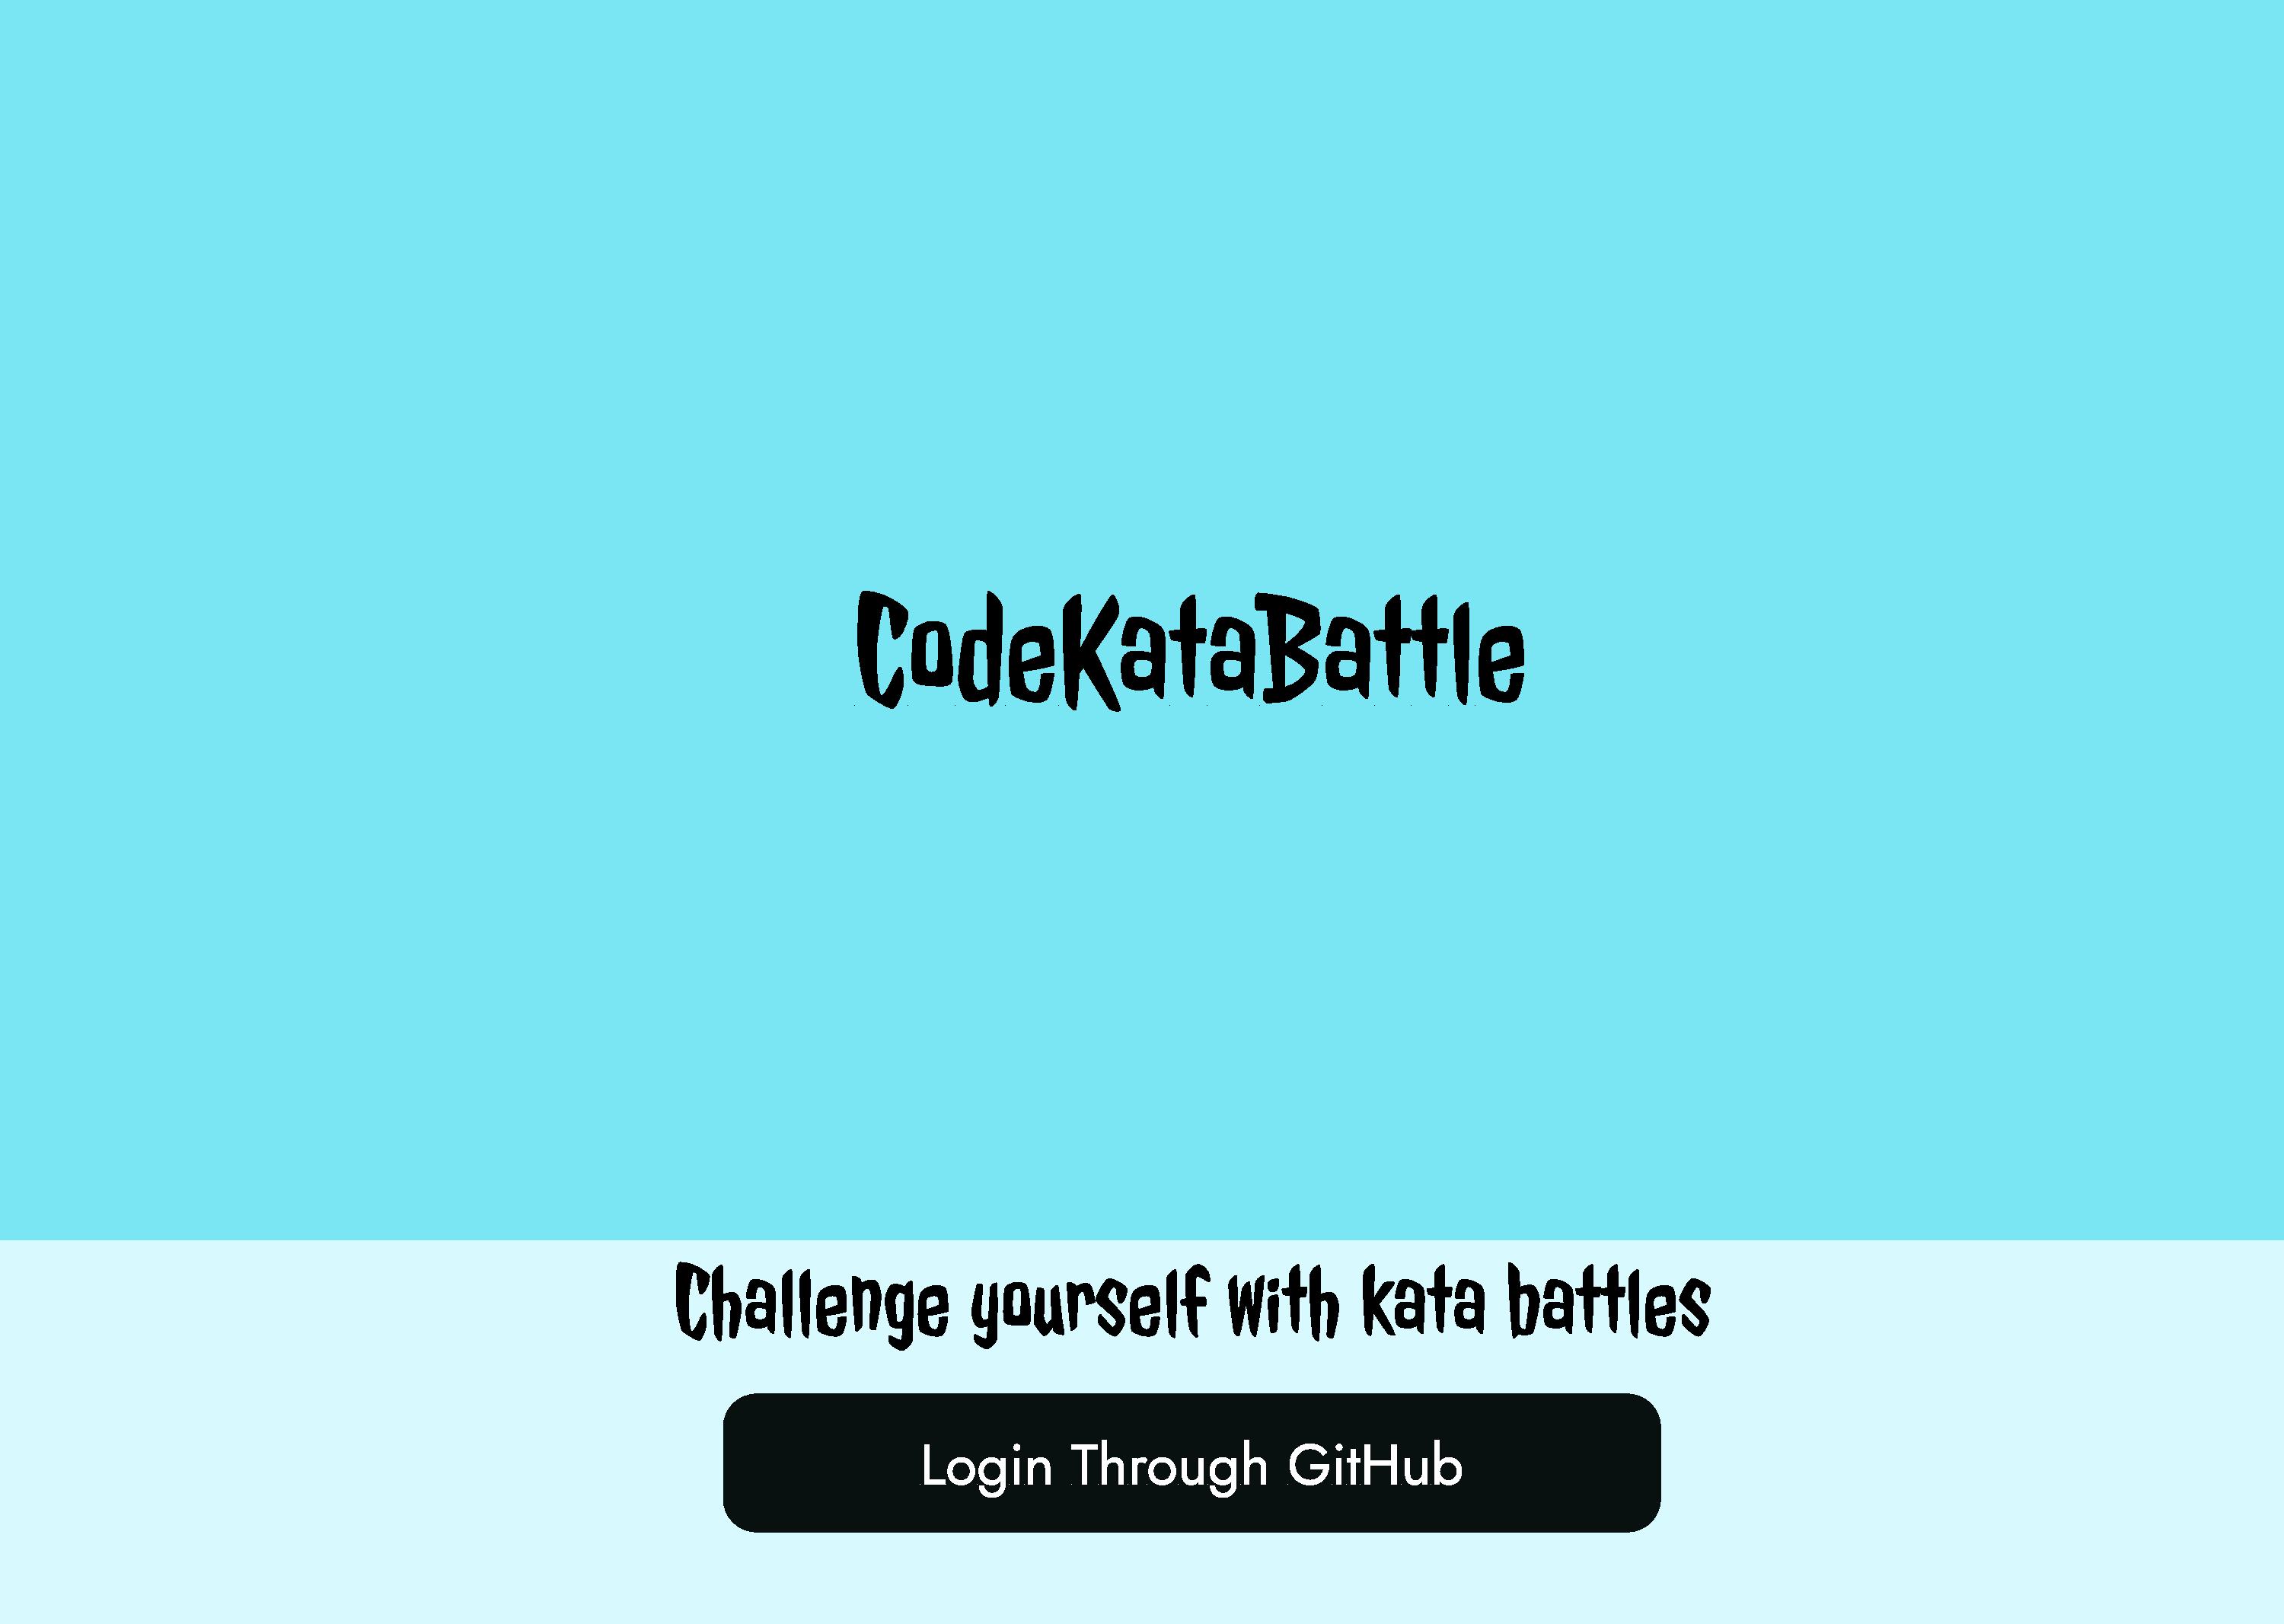
\includegraphics[page=1,width=0.7\linewidth,keepaspectratio]{3Specific_Requirements/res/UI_Mockup}

  \end{center}
    Log In Interface for both Educators and Students, who can access \app through their GitHub account by clicking on the button "Login Through GitHub"
\end{minipage}

\vspace{1cm}

\begin{minipage}{\linewidth}
	\textbf{Home Page Student}
	\begin{center}
		\includegraphics[page=2,width=0.7\linewidth,keepaspectratio]{3Specific_Requirements/res/UI_Mockup}
		
	\end{center}
	Home page for a student, in which it is possible to:
	\begin{itemize}
		\item See personal profile of the student, with a customary image.
		\item See the list of badges earned by the student in tournaments s/he participated in.
		\item Ask for the list of tournaments the student is subscribed to.
		\item Subscribe to a new tournament with the "Join Tournament" button.
		\item Search for a user on the platform (with the magnifying glass in the top right corner). 
	\end{itemize}
\end{minipage}

\vspace{1cm}

\begin{minipage}{\linewidth}
	\textbf{Home Page Educator}
	\begin{center}
		\includegraphics[page=3,width=0.7\linewidth,keepaspectratio]{3Specific_Requirements/res/UI_Mockup}
		
	\end{center}
	Home page for an educator, in which it is possible to:
	\begin{itemize}
		\item See personal profile of the educator, with a customary image.
		\item Ask for the list of tournaments the educator created (or has permissions to publish battles in), with the "My Tournaments" button.
		\item Create a new battle with the "New Battle" button. 
		\item Create a new tournament with the "New Tournament" button.
		\item Search for a user on the platform (with the magnifying glass in the top right corner). 
	\end{itemize}
\end{minipage}

\vspace{1cm}

\begin{minipage}{\linewidth}
	\textbf{Tournament Creation Form}
	\begin{center}
		\includegraphics[page=4,width=0.7\linewidth,keepaspectratio]{3Specific_Requirements/res/UI_Mockup}
		
	\end{center}
 	This interface pops up when the educator clicks on "New Tournament" from the home page. Thanks to this form, all relevant parameters for the creation of a tournament can be set.

\end{minipage}

\vspace{1cm}

\begin{minipage}{\linewidth}
	\textbf{Battle Creation Form}
	\begin{center}
		\includegraphics[page=5,width=0.7\linewidth,keepaspectratio]{3Specific_Requirements/res/UI_Mockup}
		
	\end{center}
	This interface pops up when the educator clicks on "New Battle" from the home page. Thanks to this form, all relevant parameters for the creation of a battle can be set.
	
\end{minipage}